\section{The Labour Supply in Spain}\label{sec:lab_method}

\subsection{Measuring the Aggregate Labor Supply }

This article measures aggregate labour supply as the potential annual labour input available in the population, rather than as observed employment alone. The measure combines demographic composition, labour-force participation, and hours worked, allowing changes in labour supply to be linked separately to population ageing, immigration, participation behaviour, and work intensity. Let \(L\) denote aggregate labour supply. It is computed as the weighted sum of annual hours worked by age group \(a\) and birthplace status \(r\), where \(r = (\text{foreign-born, Spanish-born})\). For each birthplace group, total labour supply depends on four components: the size of the population \(pop_{r}\), the age structure of that population \(str_{ar}\), the labour-force participation rate \(wpx_{ar}\), and annual hours worked among employed individuals \(whx_{ar}\). Formally:

\begin{equation}\label{eq:pclab}
  L = \displaystyle\sum_{r}\displaystyle\sum_{a}(pop_{r} \times str_{ar} \times wpx_{ar} \times whx_{ar}) = f(pop_{r}, str_{ar}, wpx_{ar}, whx_{ar})
\end{equation}

This formulation has two advantages. First, expressing labour supply in hours captures changes in work intensity that are missed by measures based only on population or labour-force counts. Second, using participation rates rather than employment alone includes both employed and unemployed individuals who are attached to the labour market. The resulting measure therefore ispotential labour supply rather than realised labour demand. This distinction is important because observed employment reflects the quantity of labour absorbed by the market, but not the full amount of labour available from workers. The assumption here is that unemployed individuals are willing and available to work the average annual hours observed among employed individuals of the same age group and birthplace status. Under this assumption, equation \eqref{eq:pclab} provides a consistent framework for decomposing changes in aggregate labour supply into demographic, behavioural, and work-intensity components. While this assumption make sense for demographic decompositon it's not trivial from an economique perspective, expeciespecially in Spain, where long-term unemployment and skill mismatch are structural. Therefore the estimation from \eqref{eq:pclab} is a potential labour supply measure, not a welfare-relevant or market-clearing concept. Table \ref{tab:labSum} summarizes the size of the population aged 16 and over and the corresponding aggregate labour supply in 2005 and 2025.


\begin{table}[H]%
  \caption{Population and aggregate labour supply by birthplace, Spain, 2005 and 2025.}

  %\source{Author's calculations}
  \label{tab:labSum}%
  \begin{center}
    \input{../resrc/labSum.tex}%
    \caption*{\small Note: Population is reported in millions. Aggregate labour supply is reported in millions of full-time equivalent (FTE) workers, where one FTE corresponds to 2,000 annual hours worked.}
  \end{center}
\end{table}%


Table \ref{tab:labSum} provides a first overview of population and aggregate labour supply by birthplace status, comparing levels in 2005 and 2025 with the net change over the period. Between 2005 and 2025, Spain’s population aged 16 and over increased by \(5.53\) million, from \(36.58\) to \(42.11\) million. This growth was driven mainly by the foreign-born population, which increased by \(4.74\) million, compared with only \(0.79\) million among the Spanish-born. Aggregate labour supply rose by \(2.18\) million FTE workers over the same period. This increase came entirely from the foreign-born population, whose labour supply grew by \(3.04\) million FTE workers, while Spanish labour supply declined by \(0.86\) million.

\vspace{0.7em}\par
This measure captures \emph{potential} labour supply, as it is based on labour-force participation rather than employment alone. Since foreign-born individuals typically face higher unemployment rates than natives, an employment-only measure would imply a smaller and more cyclical foreign-born contribution, especially during downturns. The present approach therefore abstracts from short-run labour-demand constraints to isolate demographic and behavioural drivers of aggregate labour supply. The next subsection examines how these aggregate changes are reflected in the age composition of the population



\subsection{Age Composition and Labour-Supply}

\begin{figure}[H]%
  \caption{Relative weight of major age groups in the population aged 16 and over and in the aggregate labor supply, and change in percentage points (pp), Spain 2005-2025}
  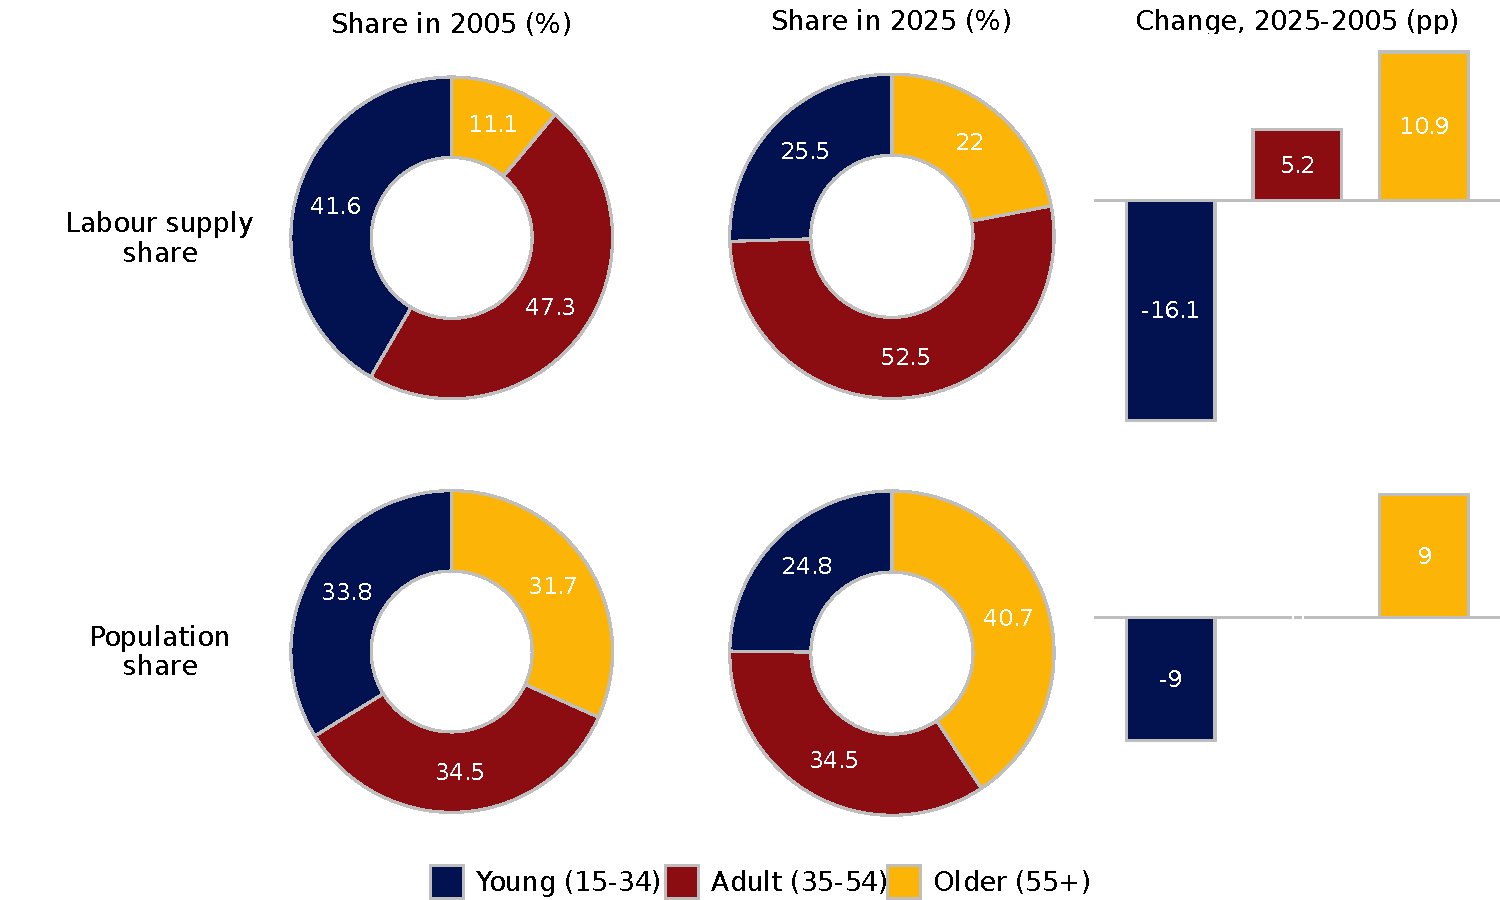
\includegraphics[width=1\textwidth]{../resrc/labPopChg.pdf}%
  \label{fig:labPopChg}%
\end{figure}%


Between 2005 and 2025, Spain’s labour supply shifted strongly away from young workers and toward older and prime-age workers. The young group, aged 15-34, declined from 41.6\% to 25.5\% of aggregate labour supply, a fall of 16.1 percentage points. This drop is much larger than their population-share decline of 9.0 percentage points, suggesting that demographic change alone does not explain the fall. Older workers, aged 55+, moved in the opposite direction. Their population share increased by 9.0 percentage points, from 31.7\% to 40.7\%, but their labour-supply share increased even more, from 11.1\% to 22.0\%, a rise of 10.9 percentage points. This implies that older individuals are contributing more to labour supply not only because they are more numerous, but also because they are more attached to the labour market than before. This behavioral change regarding labour attachment is even more prevalent among the prime-age adults whose contribution to the employment has increased by 5pp despite no change in their population share. In short, Spain’s ageing population does not mechanically reduce aggregate labour supply. The figure shows that behavioural changes, especially higher labour-market contribution among older and prime-age adults, partly offset demographic ageing, while the sharp decline among young workers reflects both demographic shrinkage and weaker labour-supply attachment. And to this, immigration has played a decisive role, as the next figure will show.



\subsection{Labour-Supply Growth by Age and Birthplace}

\begin{figure}[H]%
  \caption{Trend of the aggregate labor supply as a percentage of its level at the beginning of the period, by age group for spanish and immigrants, Spain 2005-2025}
  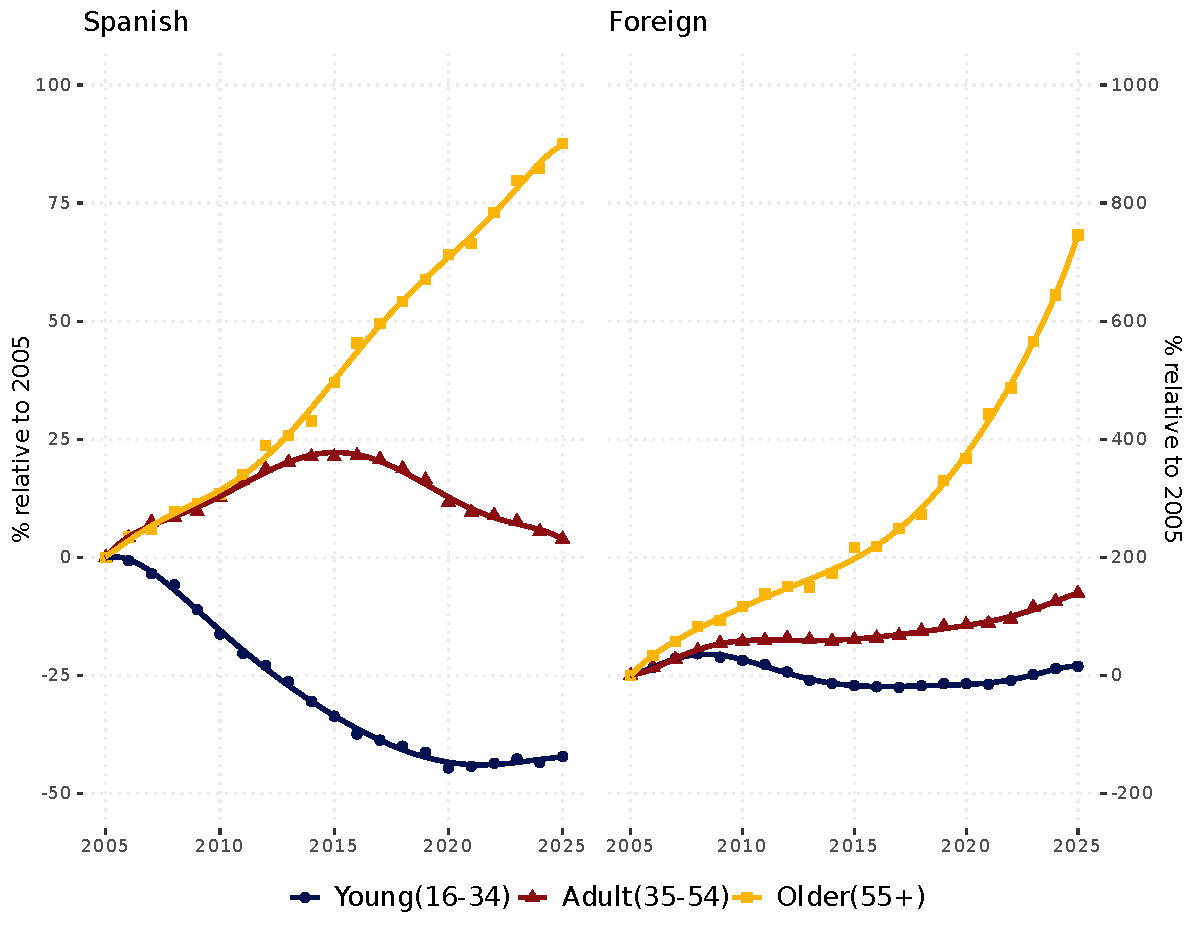
\includegraphics[width=1\textwidth]{../resrc/labRate.pdf}%
  \label{fig:labRate}%
\end{figure}%


The figure shows that immigration is the main source of labour-supply growth, especially among older and prime-age workers. For Spanish, young workers aged 15-34 show a persistent decline in labour supply, falling about 42.2\% below their 2005 level by 2025. Prime-age Spanish aged 35-54 increased until the mid-2010s but returned close to the 2005 level by 2025, only 3.9\% higher. The only strong sustained increase among Spanish is for older workers aged 55+, whose labour supply rose by 87.6\%. For foreigners, the pattern is much more expansionary. Foreign prime-age labour supply increased by 138.9\% relative to 2005, and foreign older labour supply rose by 745.9\%. Young foreign workers are more volatile: they rose before the financial crisis, declined after 2008, and recovered to 15.5\% above the 2005 level by 2025. In short, the figure suggests that Spain’s aggregate labour-supply adjustment is not driven only by ageing among natives. Immigration plays a decisive role by expanding the labour contribution of foreign adults and, especially, older foreign workers, while young native labour supply continues to contract.













